


\tikzset{every picture/.style={line width=0.75pt}} %set default line width to 0.75pt        

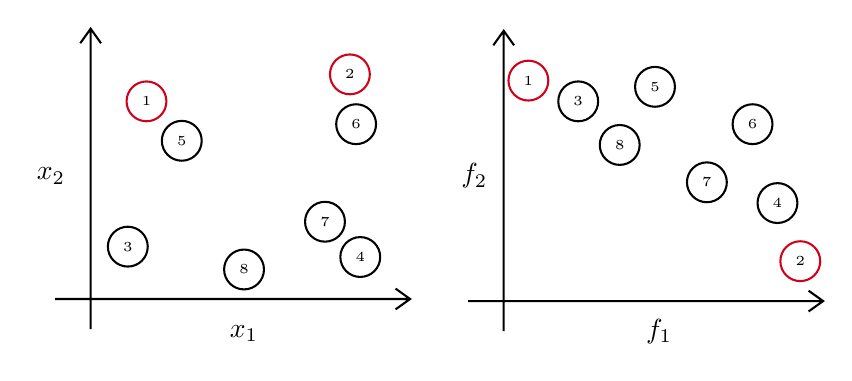
\begin{tikzpicture}[x=0.75pt,y=0.75pt,yscale=-1,xscale=1]
%uncomment if require: \path (0,340.9375); %set diagram left start at 0, and has height of 340.9375

%Shape: Axis 2D [id:dp3645341276574614] 
\draw  (50,200.22) -- (221,200.22)(67.1,70) -- (67.1,214.69) (214,195.22) -- (221,200.22) -- (214,205.22) (62.1,77) -- (67.1,70) -- (72.1,77)  ;
%Shape: Axis 2D [id:dp14963900792703488] 
\draw  (249,201.22) -- (420,201.22)(266.1,71) -- (266.1,215.69) (413,196.22) -- (420,201.22) -- (413,206.22) (261.1,78) -- (266.1,71) -- (271.1,78)  ;

% Text Node
\draw  [color={rgb, 255:red, 208; green, 2; blue, 27 }  ,draw opacity=1 ]  (94, 105) circle [x radius= 9.6, y radius= 9.6]   ;
\draw (94,105) node  [font=\tiny] [align=left] {1};
% Text Node
\draw  [color={rgb, 255:red, 0; green, 0; blue, 0 }  ,draw opacity=1 ]  (111, 124) circle [x radius= 9.6, y radius= 9.6]   ;
\draw (111,124) node  [font=\tiny] [align=left] {5};
% Text Node
\draw  [color={rgb, 255:red, 208; green, 2; blue, 27 }  ,draw opacity=1 ]  (192, 92) circle [x radius= 9.6, y radius= 9.6]   ;
\draw (192,92) node  [font=\tiny] [align=left] {2};
% Text Node
\draw    (195, 116) circle [x radius= 9.6, y radius= 9.6]   ;
\draw (195,116) node  [font=\tiny] [align=left] {6};
% Text Node
\draw  [color={rgb, 255:red, 0; green, 0; blue, 0 }  ,draw opacity=1 ]  (180, 163) circle [x radius= 9.6, y radius= 9.6]   ;
\draw (180,163) node  [font=\tiny] [align=left] {7};
% Text Node
\draw    (197, 180) circle [x radius= 9.6, y radius= 9.6]   ;
\draw (197,180) node  [font=\tiny] [align=left] {4};
% Text Node
\draw    (141, 186) circle [x radius= 9.6, y radius= 9.6]   ;
\draw (141,186) node  [font=\tiny] [align=left] {8};
% Text Node
\draw    (85, 175) circle [x radius= 9.6, y radius= 9.6]   ;
\draw (85,175) node  [font=\tiny] [align=left] {3};
% Text Node
\draw  [color={rgb, 255:red, 208; green, 2; blue, 27 }  ,draw opacity=1 ]  (278, 95) circle [x radius= 9.6, y radius= 9.6]   ;
\draw (278,95) node  [font=\tiny] [align=left] {1};
% Text Node
\draw  [color={rgb, 255:red, 0; green, 0; blue, 0 }  ,draw opacity=1 ]  (339, 98) circle [x radius= 9.6, y radius= 9.6]   ;
\draw (339,98) node  [font=\tiny] [align=left] {5};
% Text Node
\draw  [color={rgb, 255:red, 208; green, 2; blue, 27 }  ,draw opacity=1 ]  (409, 182) circle [x radius= 9.6, y radius= 9.6]   ;
\draw (409,182) node  [font=\tiny] [align=left] {2};
% Text Node
\draw    (386, 116) circle [x radius= 9.6, y radius= 9.6]   ;
\draw (386,116) node  [font=\tiny] [align=left] {6};
% Text Node
\draw  [color={rgb, 255:red, 0; green, 0; blue, 0 }  ,draw opacity=1 ]  (364, 144) circle [x radius= 9.6, y radius= 9.6]   ;
\draw (364,144) node  [font=\tiny] [align=left] {7};
% Text Node
\draw    (398, 154) circle [x radius= 9.6, y radius= 9.6]   ;
\draw (398,154) node  [font=\tiny] [align=left] {4};
% Text Node
\draw    (322, 126) circle [x radius= 9.6, y radius= 9.6]   ;
\draw (322,126) node  [font=\tiny] [align=left] {8};
% Text Node
\draw    (302, 105) circle [x radius= 9.6, y radius= 9.6]   ;
\draw (302,105) node  [font=\tiny] [align=left] {3};
% Text Node
\draw (141,217) node    {$x_{1}$};
% Text Node
\draw (48,141) node    {$x_{2}$};
% Text Node
\draw (341,216) node    {$f_{1}$};
% Text Node
\draw (252,141) node    {$f_{2}$};


\end{tikzpicture}
